\documentclass[border=10pt]{standalone}
\usepackage{pgfplots}
\pgfplotsset{compat=1.18}
\begin{document}
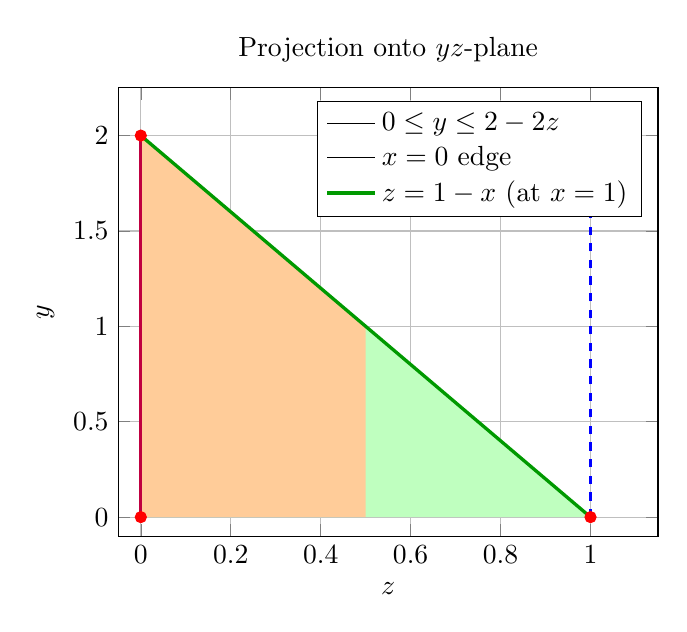
\begin{tikzpicture}
\begin{axis}[
    xlabel={$z$}, ylabel={$y$},
    xmin=-0.05, xmax=1.15, ymin=-0.1, ymax=2.25,
    grid=major,
    title={Projection onto $yz$-plane},
    legend pos=north east, legend cell align=left,
]
% Full triangle: 0<=y<=2-2z
\addplot[fill=green!25, draw=none, domain=0:1] {2-2*x} \closedcycle;
% cross-section at x=0.5: 0<=z<=0.5
\addplot[fill=orange!40, draw=none, domain=0:0.5] {2-2*x} \closedcycle;
% boundary line
\addplot[green!60!black, very thick, domain=0:1] {2-2*x};
\addlegendentry{$0 \leq y \leq 2-2z$}
% x=0 edge (z=0 axis)
\addplot[purple, very thick] coordinates {(0,0) (0,2)};
\addlegendentry{$x=0$ edge}
% z=1-x for x=1
\addplot[blue, dashed, thick] coordinates {(1,0) (1,2)};
\addlegendentry{$z = 1-x$ (at $x=1$)}
% vertices
\addplot[only marks, mark=*, color=red] coordinates {(0,0) (0,2) (1,0)};
\end{axis}
\end{tikzpicture}
\end{document}